\documentclass[main.tex]{subfiles}
\begin{document}
\subsection{With $\left|\mu\right>=\left|\mu_1+\mu_2\right>$ the highest weight of the adjoint representation of $\mathfrak{su}(3)$ show that the states $\left|A\right>=E_{-\alpha^1}E_{-\alpha^2}\left|\mu\right>$ \& $\left|B\right>=E_{-\alpha^2}E_{-\alpha^1}\left|\mu\right>$ are linearly independent}
Consider two states $\left|x\right>, \left|y\right>$, $\exists a,b\neq0 \st a\left|x\right>+ b\left|y\right>=0 \iff\left|x\right>, \left|y\right>$ linearly dependent and we know  $\frac{b^2}{a^2}=-1$ So $\left|x\right>= -\frac{b}{a}\left|y\right>$ and $\left|y\right>= -\frac{a}{b}\left|x\right>$. But then
\begin{equation}
\left<x|y\right>.\left<y|x\right>=-\frac{b}{a}\left<y|y\right>.\left(-\frac{a}{b}\right)\left<x|x\right>=\left<y|y\right>.\left<x|x\right>.
\end{equation}
Therefore we wish to calculate $\left<A|A\right>$, $\left<B|B\right>$, $\left<B|A\right>$ \& $\left<A|B\right>$. So, making use of $E_{\alpha}^{\dagger}=E_{-\alpha}$
\begin{align}
\left<A|A\right>&=\left<\mu|E_{\alpha^2}E_{\alpha^1}E_{-\alpha^1}E_{-\alpha^2}\mu\right>\\
\left<B|B\right>&=\left<\mu|E_{\alpha^1}E_{\alpha^2}E_{-\alpha^2}E_{-\alpha^1}|\mu\right>
\end{align}
\begin{align}
\left<A|B\right>&=\left<\mu|E_{\alpha^2}E_{\alpha^1}E_{-\alpha^2}E_{-\alpha^1}|\mu\right>\\
&=\left<\mu|([E_{\alpha^2},E_{\alpha^1}]+E_{\alpha^1},E_{\alpha^2})E_{-\alpha^2}E_{-\alpha^1}|\mu\right>\\
&=\left<B|B\right> + \left<\mu|\left(\left[[E_{\alpha^2},E_{\alpha^1}],E_{-\alpha^2}\right]+E_{-\alpha^2}[E_{\alpha^2},E_{\alpha^1}]\right)E_{-\alpha^1}|\mu\right>\\
&=\left<B|B\right> +
\left<\mu\right|\big(\left[\left[\left[E_{\alpha^2},E_{\alpha^1}\right],E_{-\alpha^2}\right],E_{-\alpha^1}\right] +E_{-\alpha^1}[[E_{\alpha^2},E_{\alpha^1}],E_{-\alpha^2}] \nonumber\\      &\quad+E_{-\alpha^2}[[E_{\alpha^2},E_{\alpha^1}],E_{-\alpha^1}]  +E_{-\alpha^2}E_{-\alpha^1}[E_{\alpha^2},E_{\alpha^1}]
\big)\left|\mu\right>\label{eq:9.1}
\end{align}
So \eqref{eq:9.1} is equal to $\left<B|B\right> + \text{non-vanishing terms}$, they are all non-vanishing because $\alpha^1$, $\alpha^2$ \& $\alpha^1+\alpha^2$ are all roots of the adjoint representation of $\mathfrak{su}(3)$. It can also be shown that 
\begin{equation}
\left<B|A\right>=\left<A|A\right> + \text{non-vanishing terms}.
\end{equation}
and therefore that
\begin{equation}
\left<A|A\right>\left<B|B\right>\neq \left<B|A\right> \left<A|B\right>
\end{equation}
thus the states are linearly independent.

\subsection{Show the the matrices $\frac{1}{2}\lambda_a\otimes\sigma_2$, $a=1,3,4,6,8$ and $\frac{1}{2}\lambda_a\otimes\mathbb{I}$, $a=2,5,7$ generate a reducible representation of $\mathfrak{su}(3)$ and reduce it.}
The commutation relations
\begin{align}
\frac{1}{4}[\lambda_a\otimes\sigma_2,\lambda_b\otimes\sigma_2]&=\frac{1}{2}\img f_{abc}\lambda_c\otimes\mathbb{I},\\ \frac{1}{4}[\lambda_a\otimes\mathbb{I},\lambda_b\otimes\sigma_2]&=\frac{1}{2}\img f_{abc}\lambda_c\otimes\sigma_2,\\
\frac{1}{4}[\lambda_a\otimes\mathbb{I},\lambda_b\otimes\mathbb{I}]&=\frac{1}{2}\img f_{abc}\lambda_c\otimes\mathbb{I}.
\end{align}

We pick $H_1=\frac{1}{2}\lambda_3\otimes\sigma_2$ and $H_2=\frac{1}{2}\lambda_8\otimes\sigma_2$ as the Cartan subalgebra. Using the general result that for the tensor product of two matrices $A\otimes B$ their eigenvalues multiply ${(\Lambda_{A\otimes B})}_{i,j}={(\Lambda_{A})}_i{(\Lambda_{B})}_j$ Then the eigenvalues of $H_1$ and $H_2$ are $(\pm\frac{1}{2}, 0)$ and $(\pm\frac{\sqrt{3}}{3}, \pm\frac{\sqrt{3}}{6})$ respectively. The eigenvectors are given by the eigenvectors of $\sigma_2$, $V_{\pm}=\begin{pmatrix}1\\\pm\img\end{pmatrix}$in the various spaces. Therefore the eigenvectors and their associated weights are
\begin{align}
\begin{pmatrix}V_{\pm}\\0\\0\end{pmatrix}\rightarrow(\pm\frac{1}{2},\pm\frac{\sqrt{3}}{6})\quad \begin{pmatrix}0\\V_{\pm}\\0\end{pmatrix}\rightarrow(\pm\frac{1}{2},\pm\frac{\sqrt{3}}{6})\quad
\begin{pmatrix}0\\0\\V_{\pm}\end{pmatrix}\rightarrow(0,\pm\frac{\sqrt{3}}{3}).
\end{align}

Plotting the weight diagram 
\begin{figure}[H]
\centering
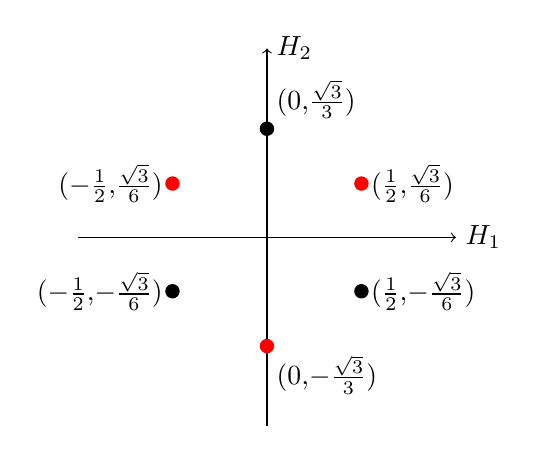
\begin{tikzpicture}[scale=1.2]
\draw[->] (0,-2) -- (0,2) node[right] {$H_2$};
\draw[->] (-2,0) -- (2,0) node[right] {$H_1$};
\filldraw[red] (1,0.57) circle (2pt) node[right, black] {($\frac{1}{2}$,$\frac{\sqrt{3}}{6}$)};
\filldraw[black] (1,-0.57) circle (2pt) node[right] {$(\frac{1}{2}$,$-\frac{\sqrt{3}}{6})$};
\filldraw[red] (-1,0.57) circle (2pt) node[left, black] {$(-\frac{1}{2}$,$\frac{\sqrt{3}}{6})$};
\filldraw[black] (-1,-0.57) circle (2pt) node[left] {$(-\frac{1}{2}$,$-\frac{\sqrt{3}}{6})$};
\filldraw[black] (0,1.15) circle (2pt) node[above right] {$(0$,$\frac{\sqrt{3}}{3})$};
\filldraw[red] (0,-1.15) circle (2pt) node[below right, black] {$(0$,$-\frac{\sqrt{3}}{3})$};
\end{tikzpicture}
\end{figure}
So the representation reduces to $3\oplus\bar3$.


\subsection{Decompose the $3\otimes3$ tensor product of $\mathfrak{su}(3)$}
Suppose $D_1$, $D_2$ irreps of $\mathfrak{su}(3)$ on $V_1, V_2$ with $V=V_1\otimes V_2$. $D=D_1\otimes\mathbb{I}+\mathbb{I}\otimes D_2$ the tensor product rep on $V$, which is not necessarily an irrep on $V$. In a basis of $V_1$, $V_2$ consisting of eigenstates of the Cartan generators $D_1(H_1),D_1(H_2),D_2(H_1),D_2(H_2)$, then for some state $\left|\phi_i\right>\in V_i$ a linear combination of basis states with weight $(p_i,q_i)$. Then $D_i(H_1)\left|\phi_i\right>=p_i\left|\phi_i\right>$, $D_i(H_2)\left|\phi_i\right>=q_i\left|\phi_i\right>$. Then $D(H_1)\left|\phi\right>=D_1(H_1)\left|\phi_1\right>\otimes\left|\phi_2\right>+\left|\phi_1\right>\otimes D_2(H_1)\left|\phi_2\right>=(p_1+p_2)\left|\phi\right>$. Therefore the weight of the state $\left|\phi\right>$ is $((p_1+p_2),(q_1+q_2))$ thus the highest weight state is $(\frac{1}{2}+\frac{1}{2}, \frac{\sqrt{3}}{6}+\frac{\sqrt{3}}{6})=(1, \frac{1}{\sqrt{3}})$. Applying the raising and lowering operators $E_{\pm1,0},E_{\pm1/2,\pm\sqrt{3}/2},E_{\mp1/2,\pm\sqrt{3}/2}$. This gives the other weights $(1/2,-\sqrt{3}/6)$, $(0,1/\sqrt{3})$, $ (1/2,-\sqrt{3}/6)$, $(0,-2/\sqrt{3})$, $(-1/2,-\sqrt{3}/6)$, $ (-1,1/\sqrt{3})$, $(0,1/\sqrt{3})$, $(-1/2,-\sqrt{3}/6)$. Plotting on the weight diagram
\begin{figure}[H]
\centering
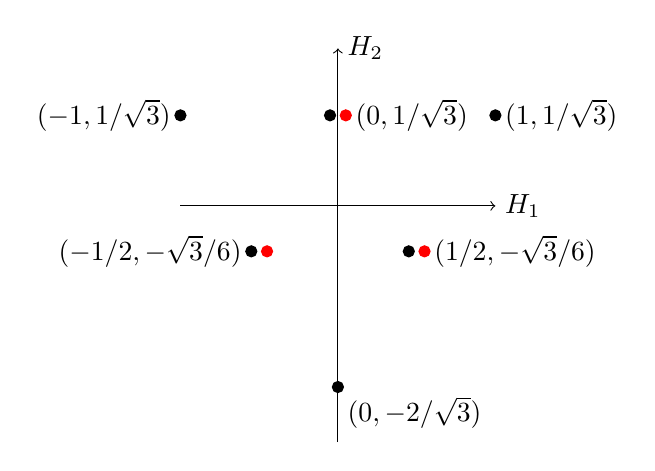
\begin{tikzpicture}
\draw[->] (0,-3) -- (0,2) node[right] {$H_2$};
\draw[->] (-2,0) -- (2,0) node[right] {$H_1$};
\filldraw[black] (2,1.15) circle (2pt) node[right, black] {$ (1,1/\sqrt{3})$};
\filldraw[black] (-2,1.15) circle (2pt) node[left, black] {$ (-1,1/\sqrt{3})$};
\filldraw[black] (0.9,-0.577) circle (2pt);
\filldraw[red] (1.1,-0.577) circle (2pt) node[right, black] {$(1/2,-\sqrt{3}/6)$};
\filldraw[black] (-0.1,1.15) circle (2pt);
\filldraw[red] (0.1,1.15) circle (2pt) node[right, black] {$(0,1/\sqrt{3})$};
\filldraw[black] (0,-2.3) circle (2pt) node[below right, black] {$(0,-2/\sqrt{3})$};
\filldraw[black] (-1.1,-0.577) circle (2pt) node[left, black] {$ (-1/2,-\sqrt{3}/6)$};
\filldraw[red] (-0.9,-0.577) circle (2pt) ;
\end{tikzpicture}
\end{figure}
Thus we see that the weights $(\pm1/2,-\sqrt{3}/6)$ and $(0,-1/\sqrt{3})$ have multiplicity 2 and therefore the $3\otimes3$ tensor product representation is not irreducible on the 9-dimensional vector space. The state with multiplicity 2 correspond to the $\bar3$ representation of $\mathfrak{su}(3)$ while the remianing states correspond to the $6$ and therefore we see the decomposition $3\otimes3=6\oplus\bar3$
\end{document}